\documentclass[
fontsize=10pt, % Base font size
twoside=false, % If true, use different layouts for even and odd pages (in particular, if twoside=true, the margin column will be always on the outside)
%abstract=true, % Uncomment to print the title of the abstract
%numbers=noenddot, % Comment to output dots after section numbers; the most common values for this option are: enddot, noenddot and auto (see the KOMAScript documentation for an in-depth explanation)
%draft=true, % If uncommented, rulers will be added in the header and footer
%overfullrule=true, % If uncommented, overly long lines will be marked by a black box; useful for correcting spacing problems
]{kaobook}

% Choose the language
\usepackage[english]{babel} % Load characters and hyphenation
\usepackage[english=british]{csquotes}	% English quotes

% Load the bibliography package
\usepackage{styles/kaobiblio}
\addbibresource{references.bib} % Bibliography file

%%%%%% Math packages
%\usepackage{siunitx}
\newcommand{\si}{~}  % TODO: siunitx fails 

%%%%%% definitions of mathematical variables
\newcommand{\bbf}{{\mathbf b}}
\newcommand{\ebf}{{\mathbf e}}
\newcommand{\jbf}{{\mathbf j}}
\newcommand{\kbf}{{\mathbf k}}
\newcommand{\ubf}{{\mathbf u}}
\newcommand{\vbf}{{\mathbf v}}
\newcommand{\xbf}{{\mathbf x}}
\newcommand{\Bbf}{{\mathbf B}}
\newcommand{\Ebf}{{\mathbf E}}
\newcommand{\Mbf}{{\mathbf M}}
\newcommand{\Sbf}{{\mathbf S}}
\newcommand{\Vbf}{{\mathbf V}}
\newcommand{\nablabf}{\mbox{\boldmath${\nabla}$}}


%%%%%% numerote aussi les subsections
\setcounter{secnumdepth}{3}


%%%%%% section and subsection properties
\usepackage{titlesec}
\usepackage{sectsty}
% set section/subsections HEADINGS font and color
\definecolor{ColorSection}{rgb}{0.8,0.0,0.0} %mix personal color
\definecolor{ColorSubSection}{rgb}{0.2,0.4,0.6} %mix personal color
\sectionfont{\color{ColorSection}}  % sets colour of sections
\subsectionfont{\color{ColorSubSection}}  % sets colour of subsections


%%%%%%%%%%%%%%%%%%%%%%%%%%%%%%%%%%%%%%%%%%%%%%%%
\title{Tokamak Dimensioning}
\subtitle{Lecture, Master on Fusion Science}

\author{J. Hillairet, Y. Sarazin, J.-L. Duchateau et al.}
\date{\today}

%\frontmatter % Denotes the start of the pre-document content, uses roman numerals

\begin{document}

\maketitle

\setcounter{tocdepth}{4}
\tableofcontents

\mainmatter % Denotes the start of the main document content, resets page numbering and uses arabic numbers
\setchapterstyle{kao} % Choose the default chapter heading style, for kaobook only

\newpage
% -------------------------------------------------------------
% -------------------------------------------------------------
\section{Introduction}
\margintoc
% -------------------------------------------------------------
\subsection{Work objectives}
Why is ITER so large? How have been determined its main dimensions? Are these dimensions sufficient to reach its scientific goals,  i.e. produce 500 MW of fusion power for pulses of 400s with a power amplification ratio of 10\marginnote{\url{https://www.iter.org/sci/Goals}}? And what should be the size of tokamak fusion reactor: smaller or larger than ITER? How much additional power is required to reach positive power amplification? How does it affect the magnets and the plasma facing components? Should a fusion reactor be larger than ITER?

Answering these questions is the main motivation for this group work. During the few days dedicated to this work, you will have to answers some of these questions by working in small groups. Interactions between groups is highly encouraged: no one can be expert of all the various physical and technological fields required to build a fusion machine, so group work is essential. When necessary, results will be shared between groups.

\begin{marginfigure}[-3.8cm]
	\centering
	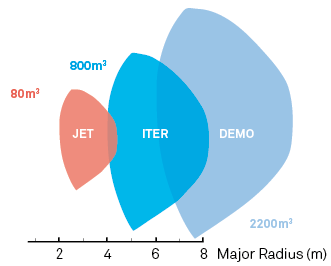
\includegraphics[width=1\linewidth]{figures/size_JET_ITER_DEMO}
	\caption{Size of present and future tokamaks.}
	\label{fig:sizejetiterdemo}
\end{marginfigure}

In the first part of the work, you will derive from a 0-dimensional approach the necessary equations to deduce a couple $(R_0, B_0)$ for a given reactor project of prescribed $(P_{DT}, Q)$. By proceeding this way, some other characteristics of the plasma (namely the shape of the plasma, including elongation and aspect ratio, the average ion mass $\hat M$, the edge safety factor $q_a$ and the density $n_N$ normalized to the Greenwald density $n_G$) will have to be prescribed by other considerations. This method will be applied to deduce the ITER parameters $(R_0, B_0)$. 

Each group results will be presented and shared with each others during the Part 1 evaluation. Once done, you will have to fix the main dimensions of the tokamak to be build. In the Part 2, groups will then focus on particular aspects of the machine: magnets, MHD stability, plasma facing components, safety and remote handling, external heating systems, etc. In case of problems, questions or design change requests, groups will be able to exchange between each other, or even to organise a general meeting in which topics affecting all groups can be discussed.

% --------------------------------------------
\subsection{Preamble on Units}
The International System of Units (SI) should be used. Quantities which are \emph{not} expressed in SI units should be emphasized with a specific symbol, for example with hats ``$\hat{...}$''. We recommand using the following alternative units:

\begin{itemize}
	\item $\hat n$ is the density in $10^{19} \si{m^{-3}}$: 
	$\hat n = 10^{-19}\,n_{\si{[m^{-3}]}}$
	\item $\hat T$ is the temperature in $keV$: $\hat T = 10^{-3}\, k_B T_{[K]}\,/e$ \\(with $k_B \approx 1.3807\, 10^{-23} \si{J.K^{-1}}$ the Boltzmann's constant and $e\approx 1.6022\, 10^{-19}C$ the elementary electric charge)
	\item $\hat I_p$ is the plasma current in MA: $\hat I_p = 10^{-6}\,I_{p\,[A]}$
	\item $\hat P$ is the power in MW: $\hat P = 10^{-6}\, P_{[W]}$
	\item $\hat M$ is the mass in Atomic Mass Unit
\end{itemize}

When possible, try to combine all numerical values (coming from physical constants) into a single constant $C$. In a later stage, these equations will be rewritten in a convenient set of units commonly used in tokamak physics.


\subsection{Reminder: Plasma Geometry}
The usual plasma equilibrium are illustrated in figure \ref{fig:tokamakequilibrium_parameters}. If $\theta$ is the poloidal angle ($\theta=0$ on the equatorial plane), then one has the following relationships\marginnote{The circular plasma corresponds to the limit case $\kappa=1$, $\delta=0$. }:
\begin{align}
R =& R_0 + a \cos \left(\theta - \delta \sin\theta \right) \\
Z =& \kappa a \sin \theta
\end{align}
The ITER case corresponds to $R_0=6.2$ m, $a=2$ m, $\kappa=1.85$, $\delta=0.5$. 

\begin{figure}[h]
	\centering
	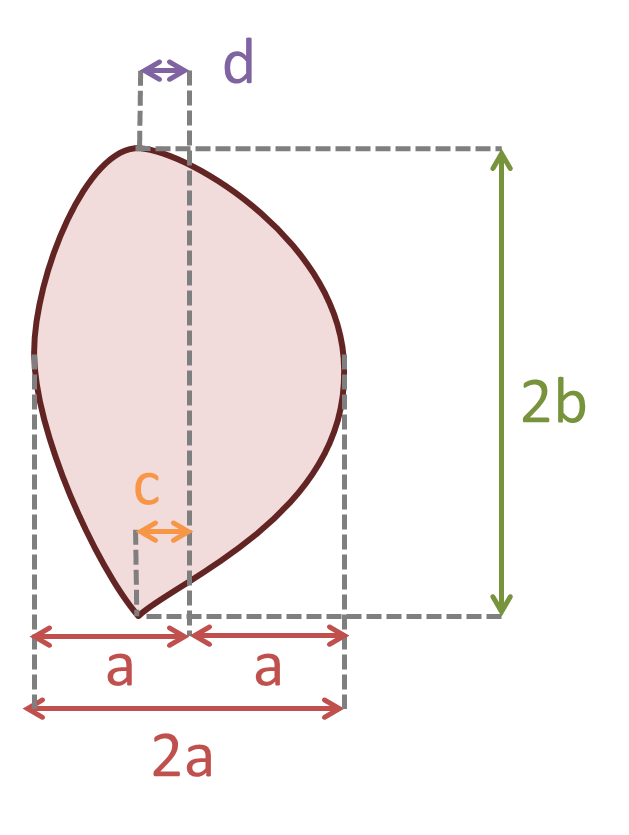
\includegraphics[width=0.39\linewidth]{figures/Tokamak_equilibrium1}
	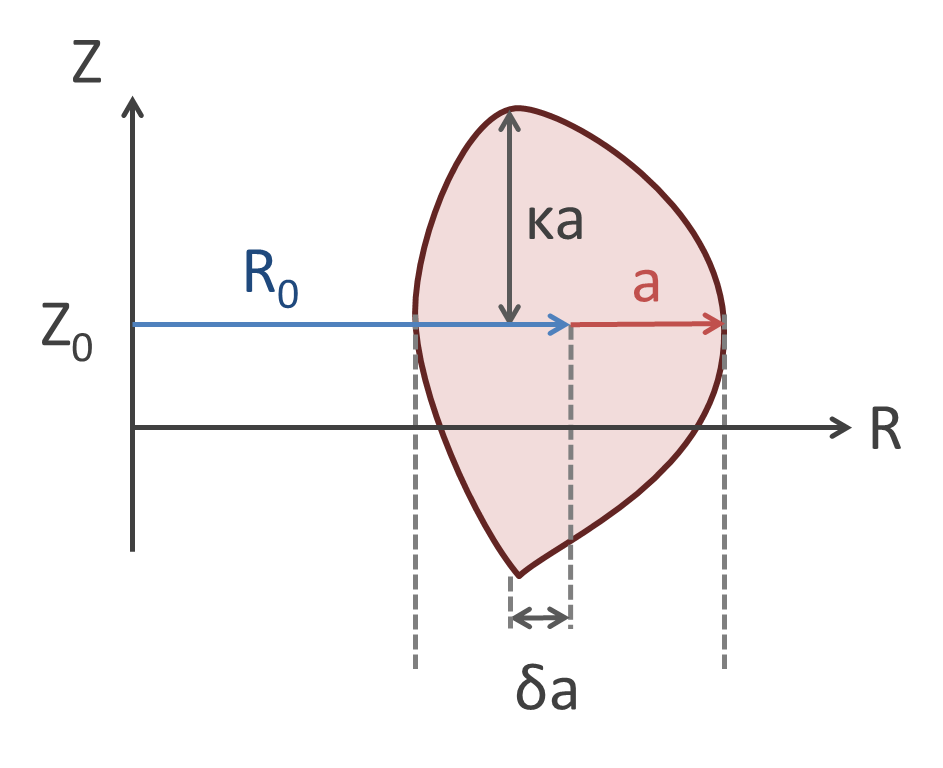
\includegraphics[width=0.59\linewidth]{figures/Tokamak_equilibrium2}
	\caption{Usual plasma equilibrium geometrical parameters. Plasma elongation: $\kappa=b/a$. Plasma triangularity: $\delta=\frac{c+d}{2a}$. }
	\label{fig:tokamakequilibrium_parameters}
\end{figure}

The volume of an elliptic tore can be approximated by:

\begin{equation}
V_t = 2\pi^2 \kappa R a^2
\end{equation}

\noindent
with $a$ the minor radius and $R$ the major radius of the tore. Here, $\kappa \doteq b/a$ stands for the \textit{elongation} of the plasma, $b$ being the largest radius of the ellipsoid (cf figure \ref{fig:tokamakequilibrium_parameters}). $\kappa=1$ for a circular cross-section, and is larger than unity for an elongated plasma.

Introducing the \textit{inverse aspect ratio} $\varepsilon$ defined as 
\begin{equation}
	\varepsilon  \doteq a /R
\end{equation}
the volume then reads:

\begin{equation}
V_t = 2\pi^2\varepsilon^2 R^3
\label{eq:tore_volume}
\end{equation}
\noindent
with $\kappa=1$. 


% -------------------------------------------------------------
% -------------------------------------------------------------
\newpage
\section{Derivation of the Governing Relations}\margintoc
The objective of this work is to deduce the main dimensioning parameters of a tokamak machine, namely the large radius $R_0$ and the magnitude of the (toroidal) magnetic field $B_0$ (on-axis, i.e. at normalized radius $\rho=0$) for a given couple of fusion power $P_{fus}$ and amplification factor $Q$. Since we are seeking two parameters, we will try to develop a 0D-approach sufficient to get two independent equations starting from the definition of $P_{fus}$ and $Q$. 





% --------------------------------------------
\subsection{Fusion Power $P_{fus}$}
\subsubsection{Fusion reactivity}
To get nuclear fusion, nuclei have to come close enough to each other. Nuclear forces can overcome their mutual electrostatic repulsion provided their distance becomes sufficiently close, in the order of $10^{-15}\si{m}$. %This would require temperatures of the order of 720 keV for head-on collisions of thermal particles to lead to fusion reactions in a classical way. Actually, quantum physics has to be taken into account in the process. 

However, both in tokamaks and in stars interiors, fusion reactions take place predominantly due to the tunnel effect. Crossing this barrier can be quantified in a probabilistic manner with the reaction rate $R$ $[\mathrm{reaction/m^3 s}]$, defined as the probability of reaction per unit time and volume. 

The reaction rate between mono-energetic ions of density $n_1$ $\mathrm{[m^{-3}]}$ striking target ions of density $n_2$ $\mathrm{[m^{-3}]}$ is proportional to the effective cross-section\marginnote{The cross-section is expressed as a surface quantity and measures the probability of a reaction from a single nucleus target.} area $\sigma$ $\mathrm{[m^2]}$ and to the velocity difference $v_{12}$ between the two species:

\begin{equation*}
r_{12} = n_1 n_2 \; \sigma v_{12}
\end{equation*}

The quantity $\sigma v_{12}$, which depends on the kinetic energy of the colliding particles, is called the reactivity ($\mathrm{[m^3/s]}$). Note that the reaction rate $r_{12}$ is proportional to the square of the density of the mixture. 

In fusion plasmas, ions are not mono-energetic. They are assumed to have Maxwellian velocity distributions. The average reactivity $\langle \sigma v \rangle_{12}$ derives from the following expression:

\begin{equation*}
\left < \sigma v \right >_{12} 
= \int_{-\infty}^{+\infty} \int_{-\infty}^{+\infty} 
\sigma(v_{12}) v_{12}\;  f_1(v_1) f_2(v_2) \; dv_1dv_2
\end{equation*}

Finally, the average reaction rate $R_{12}$ reads:

\begin{equation*}
R_{12} = n_1 n_2 \; \left < \sigma v \right >_{12}
\end{equation*}

It governs the time evolution of both densities: $dn_1/dt = dn_2/dt = -R_{12}$.

\begin{marginfigure}[-3.8cm]
	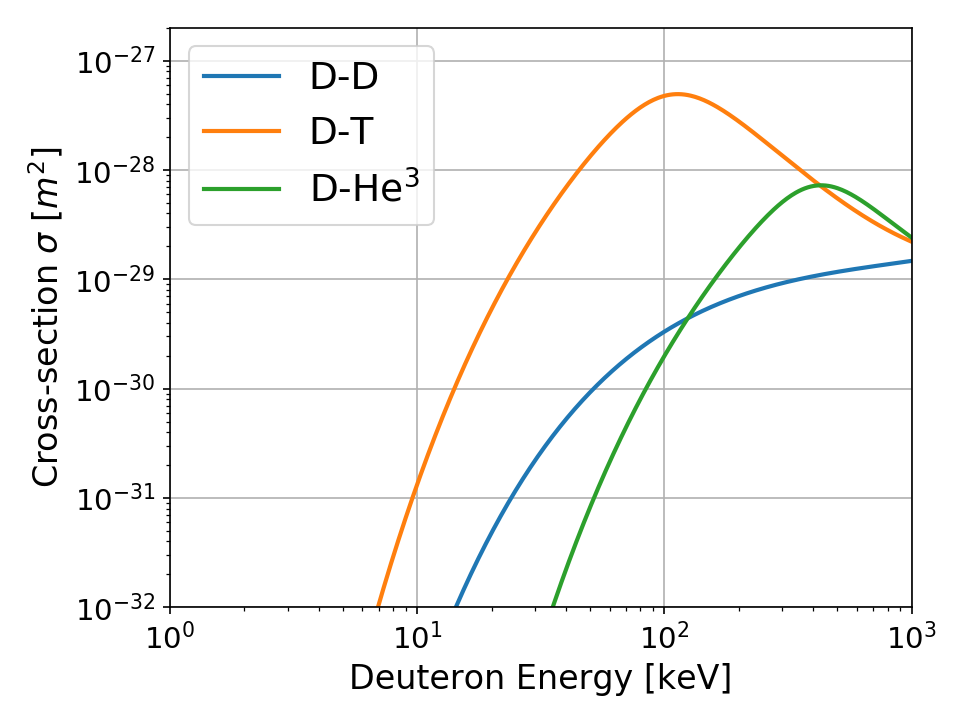
\includegraphics[width=1\textwidth]{figures/Fusion_cross-section.png}
	\caption{Fusion reactions cross-sections, data taken from \cite{Huba2013} }
	\label{fig:crosssection_adv}
\end{marginfigure}

The reactivity depends of the temperature and its evolution is known from the measurements of the cross-sections. The temperature dependence of the reactivity $\langle \sigma v \rangle_{12}$ is plotted on figure \ref{fig:reactivity_adv} for several fusion reactions (interpolated data from \sidecite{Huba2013}). 

\begin{figure}
	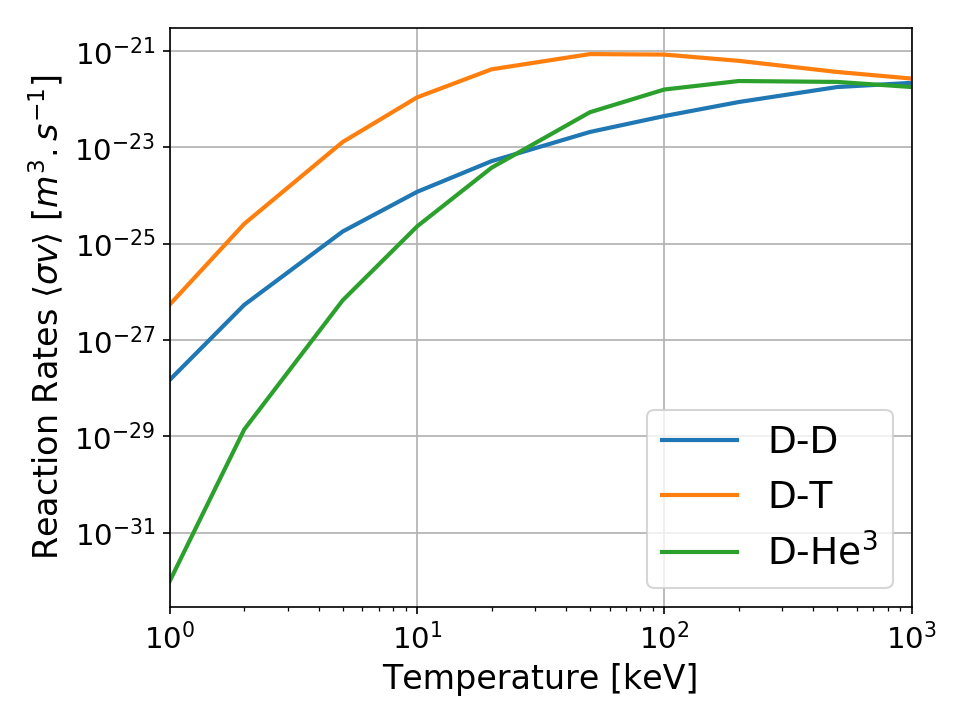
\includegraphics[width=1\textwidth]{figures/Fusion_Reactivity.png}
	\caption{Fusion reactions reactivity, data taken from \cite{Huba2013} }
	\label{fig:reactivity_adv}
\end{figure}

Of course, there is interest in operating a fusion reactor at the lowest temperatures. Looking to the figure \ref{fig:reactivity_adv}, the mixture D-T seems the "easiest" way to initiate fusion reactions, since the D-T reaction  has the maximum reactivity at lowest temperature of all fusion reactions. The D-T reactivity reaches its maximum for a temperature of 64 keV, corresponding to a temperature of $742\,10^6$ K. The D-T reaction is \sidecite{FusionCEA1987}: 

\begin{equation*}
    \mathrm{D + T} \longrightarrow \mathrm{{}^4 He~(3.56~MeV) + n~(14.03~MeV)}
\end{equation*}

The D-T reaction leads to a total released energy of $E_{DT}$ = 17.59 \si{MeV} = $2.82\times 10^{-12} \si{J}$ per fusion reaction\sidenote{This value can be compared to the 200 MeV released by $^{235}$U fission. Yet, the energy release \emph{per nucleon} ($i.e.$ per kilogram) is approximately 4 times larger for fusion than for fission reactions.}. Notice that the ratio of the total energy to that carried by the alpha particles $\lambda \doteq 17.59/3.56 \approx 4.94$ is not exactly equal to 5 as one would expect on the basis of momentum conservation. Actually, this ratio \emph{is obviously} consistent with momentum conservation, as it should, provided one takes into account relativistic effects. This point is detailed in section \ref{appendix:fusion_power}.\\

The fusion power per unit volume $p_{DT}$ produced by the fusion of the nuclei of deuterium and tritium reads: 
\begin{equation*}
  p_{DT} = n_D n_T \left< \sigma v \right>_{DT} E_{DT}
\end{equation*}
with $n_D$ and $n_T$ the deuterium and tritium density and $\left< \sigma v \right>_{DT}$ the D-T reactivity. Assuming equal deuterium and tritium densities:
\begin{equation*}
  n_D = n_T = \frac{n}{2}
\end{equation*}
with $n$ the electron density, then the thermonuclear power density is:
\begin{equation*}
  p_{DT} = \frac{1}{4} n^2 \left< \sigma v \right>_{DT} E_{DT}
\end{equation*}

Assuming a constant reactivity in the plasma ("flat profile hypothesis") and using the tore volume $V$, the fusion power is: 
\begin{equation}
  P_{fus} = \frac{V}{4}
    n^2 \left< \sigma v \right>_{DT} E_{DT}
\end{equation}



% --------------------------------------------------
\subsubsection{Relationship 1: Fusion Power}
Using the tore volume eq.\ref{eq:tore_volume}, one readily obtains the fusion power:

\begin{equation}
	P_{fus} = \frac{2\pi^2}{4}
  				\varepsilon^2 R^3
				n^2 \left< \sigma v \right>_{DT} E_{DT}
	\label{eq:FusionPower1}
\end{equation}

This is the first equation relating $P_{fus}$ to the geometrical parameter $R$. However, it is not usable yet, since from figure \ref{fig:reactivity_adv}, the reactivity $\left< \sigma v \right>$ clearly depends of the temperature. It will be thus necessary for the following to define the temperature at which the machine should operate. This will be part of the physical constraints discussion in the next section. 


This total fusion power is distributed among the alpha particles and the neutrons: 
\begin{equation}
	P_{fus} 
	= 
	P_\alpha + P_n 
	= 
	\lambda \; P_\alpha
\label{eq:P_fus_Palpha}
\end{equation}
where we recall that $\lambda \approx 4.94$. Due to the mass ratio, almost 80\% of the power is carried by the neutrons. 


% --------------------------------------------------
% --------------------------------------------------
\subsection{Amplification factor $Q$}


% -------------------------------------------------------
\subsubsection{Definition of $Q$}
Let's start from definition of the plasma amplification factor. The amplification factor is defined as the ratio of the fusion power $P_{fus}$ to the external heating power supplied $P_{ext}$\cite[p.12]{Wesson2004}, \cite[(3.4)]{FusionCEA1987}:

\begin{equation}
	Q \doteq \frac{P_{fus}}{P_{ext}}
\label{eq:definition_Q}
\end{equation}

Importantly, notice that $Q$ \emph{does not} encompass -- by far -- the entire question of the energetic efficiency of a fusion reactor. Indeed, in particular, it does neither account for the energy used for cryogenic purposes (as required by the use of superconductors) nor for the conversion factor of thermal to electric energy\sidenote{This point is often misleading for the public and it is important to be factually correct. Misleading statements concerning fusion and ITER power and energy since decades have been highlighted in \href{http://news.newenergytimes.net/2017/10/06/the-iter-power-amplification-myth/}{news.newenergytimes.net(1)}. This led directly ITER to update its public information web pages on the Q-factor (cf. \href{https://www.iter.org/newsline/-/2845}{ITER Newsline}).  Cf. also the follow-up \href{http://news.newenergytimes.net/2017/12/11/evidence-of-the-iter-power-deception/}{news.newenergytimes.net(2).}}.

% ------------------------------------------
\subsubsection{Power Balance: Sources terms}
At equilibrium, sources terms equal sink terms:
\begin{equation}
	\sum_{sources} P = \sum_{loss} P
	\label{eq:power_balance_general}
\end{equation}
where the losses terms will be discussed in the next subsections.

To the contrary with neutrons which leave the plasma, charged $\alpha$~nuclei are confined by the magnetic field and should ideally transfer their energy to the main ions before being extracted\marginnote[*-1]{There are basically 2 ways for this energy transfer. Since the collision frequency scales like the velocity difference between the colliding species to the power $-3$ ($\nu_{coll,ss'}\sim n_{s'}/\Delta v_{ss'}^3$), alpha particles transfer their energy dominantly to the electrons, which are much faster due to their low inertia. Then two routes are possible for the energy transfer from the electrons to the ions. Either via collisions, or via turbulence. In the latter case, the mediator are the electrostatic plasma waves. The relative weight of those two channels is still a matter of research.}. The total -- or \emph{net} -- heating power $P_{net}$ is the sum of the auxiliary plasma heating,  $P_{ext}$, of Ohmic heating $P_\Omega$ and of alpha heating $P_\alpha$, minus the radiative losses $P_{rad}$\sidenote[][*+10]{The reason why the radiative losses are included comes from the definition of the confinement time, described in a next section.}:

\begin{equation}
	P_{net} 
	\doteq 
	P_\alpha + P_\Omega + P_{ext} - P_{rad}
\label{eq:definition_net_power}
\end{equation}

In the following, we will assume that the ohmic contribution is negligible. Radiative losses are discussed in section~\ref{sec:plasma_radiation}. For the sake of simplicity, we will replace hereafter the radiative losses by the coefficient $0\leq \gamma_{rad} \leq1$:
\begin{equation*}
P_{net} \doteq \gamma_{rad} (P_\alpha + P_{ext})
\end{equation*}

Using \ref{eq:P_fus_Palpha} and \ref{eq:definition_Q}:
\begin{equation}
\boxed{
	P_{net} 
	\doteq 
	\gamma_{rad}
	P_{fus}
	\frac{1 + Q/\lambda}{Q}
}
\label{eq:Pnet_as_Pfus_Q}
\end{equation}
Replacing $P_{fus}$ by its expression eq.\ref{eq:FusionPower1}, one finally obtains:
\begin{equation}
\boxed{
	P_{net} 
	= 
	\gamma_{rad}
	\frac{2\pi^2}{4}
	\varepsilon^2 R^3
	n^2 \left< \sigma v \right>_{DT} E_{DT}
	\frac{1+Q/\lambda}{Q}
 }
\label{eq:Pnet_QnTR_adv}
\end{equation}

Now that we have expressed the $P_{net}$ term for the source terms, one needs to express the loss terms.

% --------------------------------------------------
\subsubsection{Power Balance: Losses and Energy Confinement time $\tau_E$}

The losses origins being diverse, it is convenient to group all losses into one term $P_{loss}$\cite[p.9]{Wesson2004}:

\begin{equation}
	P_{loss} 
	\doteq 
	\frac{ W }{ \tau_E } 
\label{eq:definition_confinement_time_global}
\end{equation}
\noindent
where $W$ is the total thermal plasma energy and where we have defined $\tau_E$ as the energy confinement time, in seconds $[\si{s}]$. 

Usually, the energy confinement time $\tau_E$ is defined as the characteristic time at which this energy is lost from the plasma due to thermal transport (conduction and convection), either by collisional conduction or by turbulent thermal convection. This leads to the following (re)definition\cite[(3.2)]{FusionCEA1987}:
\begin{equation}
	P_{loss} 
	\doteq 
	P_{rad}
	+
	\frac{ W }{ \tau_E } 
\label{eq:definition_confinement_time}
\end{equation}
\noindent
which explains now why the radiative term has been put into the net power expression(\ref{eq:definition_net_power}). Note that this latter definition is consistent with the one used for the ITER scaling laws, discussed in the next sections.


% --------------------------------------------------
\subsubsection{Plasma Thermal Energy $W$}
The total internal energy of the plasma reads as follows:
\begin{equation*}
W  = \int \frac{3}{2} k_B \left( n_e T_e + n_i T_i \right ) dV 
\approx \int 3 n k_BT dV
\end{equation*}

\noindent
where the integral is performed over the plasma volume. Here, equal ion and electron temperatures have been assumed. Assuming flat density and temperature profiles and using the expression of the volume of a torus Eq.(\ref{eq:tore_volume}), the total plasma internal energy then reads:
\begin{equation}
W = 3 n k_B T V = 3 k_B (2\pi^2) \varepsilon^2  n T R^3
\label{eq:total_energy_natural_units}
\end{equation}




% --------------------------------------------------
\subsubsection{Energy Confinement Time $\tau_E$ from Scaling Laws}
Experimental results have shown that the energy time in ELMy H-mode tokamak plasmas (referred to as the ITER IPB98(y,2) scaling law Eq.(20) of \sidecite{ITERphysics_chap2}) is well represented -- the root means square error is about 15.6\% -- by the following scaling law:

\begin{equation}
	\tau_E = C_{SL} \hat M^{0.19} \kappa^{0.78} \varepsilon^{0.58} 
	\hat n^{0.41} \hat I_p^{0.93} R^{1.97} B^{0.15}  \hat P_{net}^{-0.69}
	\label{eq:scaling_law_IPB98(y,2)_adv}
\end{equation}

\noindent
with $C_{SL} = 0.0562$.


Here, $\hat I_p$ and $B$ are the plasma current and the toroidal magnetic field at the magnetic axis, respectively, $\hat n$ the line-averaged density, and $\hat M$ is the average ion mass (in Atomic Mass Unit)\sidenote{Cf. also \href{http://fusionwiki.ciemat.es/wiki/Scaling_law}{CIEMAT FusionWiki}.}. 





% --------------------------------------------------
\subsubsection{Plasma Current $I_p$}

Integrating the Maxwell-Ampère equation over the whole plasma cross-section, and using Stokes' theorem, one gets:

\begin{equation*}
\int_\mathcal{S} (\nablabf\times \Bbf) \cdot \mathbf{dS} = 
\oint_\mathcal{C} \mathbf{B} \cdot \mathbf{d\ell}
= \mu_0 \int_\mathcal{S} \jbf \cdot \mathbf{dS} = \mu_0 I_p
\end{equation*}

Neglecting the elongation of the cross-section, the equation can be approximated as follows:
$$
2\pi a B_p = \mu_0 I_p
$$

\noindent
with $B_p$ the poloidal component of the magnetic field at the separatrix. In the limit of large aspect ratios, it can be easily related to the safety factor $q_a$ at the separatrix\sidenote{Actually, $q_a$ is usually taken slightly inside the separatrix, at 95$\%$ of the poloidal magnetic flux.}:

\begin{equation*}
q_a \doteq \frac{a}{R} \frac{B_t}{B_p} 
\end{equation*}

\noindent
with $B_t$ the toroidal component of the magnetic field at the magnetic axis. Then it comes:

\begin{equation}
\hat I_p = C_I \frac{\varepsilon^2}{q_a} \; R B
\label{eq:plasma_current_adv}
\end{equation}

\noindent
where $\hat I_p$ is the current expressed in MA, and $C_I = 2\pi\, 10^{-6} /\mu_0 = 5$  ($\mu_0 = 4\pi\, 10^{-7} \si{H.m^{-1}}$).
Notice that $B_t$ has been safely replaced by $B$ since $B_p\ll B_t$ in tokamak plasmas. 

% --------------------------------------------------
\subsubsection{Relationship 2: Power Balance, the link between $Q$ and $\tau_e$}
At equilibrium\marginnote[*-1]{Should the plasma not be at equilibrium and/or be subject to significant radiative losses in the confined region, then $P_{net}$ should be replaced by $(P_{net}-dW/dt-P_{rad})$. The subtraction of $P_{rad}$ ensures the balance equation to be consistent with the retained definition of $\tau_E$.}, i.e. from (eq.\ref{eq:power_balance_general}), one has:
\begin{equation}
	P_{net} = P_{loss}
\end{equation}

Using the expressions of $P_{net}$ (\ref{eq:Pnet_QnTR_adv}) and expending $P_{loss}$ (\ref{eq:definition_confinement_time}) using expressions of $W$ (\ref{eq:total_energy_natural_units}) and $\tau_E$ (\ref{eq:scaling_law_IPB98(y,2)_adv}) leads to
\marginnote[*+1]{Remind to include the parameter $\kappa^{0.78}$ which has been removed from the confinement time scaling law into the volume constant (as $\kappa^{-0.78}$)}:

\begin{equation}
	\left(
		\gamma_{rad} P_{fus} \frac{1 + Q/\lambda}{Q}
	\right)^{0.31}
	=
	2\pi^2 C_{loss}  C_I^{-0.93} C_{SL}^{-1}
	M^{-0.19} \varepsilon^{-0.44}
  \hat n^{0.59} \hat T  q_a^{0.93} R^{0.1} B^{-1.08} 
\end{equation}

Which is the second equation relating the target $(P_{fus}, Q)$ to the machine parameters $(R,B)$. 

However, some unknowns still remain, for instance in the expression of the fusion power $P_{fus}$, which will be discussed in the next part.

% --------------------------------------------------
% --------------------------------------------------
% --------------------------------------------------
\newpage
\section{Physical Constraints}\margintoc
% --------------------------------------------------
% --------------------------------------------------
\subsection{Reactivity and Temperature range}
Without expanding the confinement time, equilibrium relationship (\ref{eq:power_balance_general}) can be written neglecting radiation using the net power (\ref{eq:Pnet_QnTR_adv}) and plasma energy (\ref{eq:total_energy_natural_units}) expressions, as:
$$
n \tau_E 
=
C_{lawson}
\frac{Q}{1+Q/\lambda}
\frac{\hat T }{\left< \sigma v \right>_{DT} }
$$ 
with $C_{lawson} = 12\times10^3 e / (\gamma_{rad} E_{DT})\approx 6.818\times10^{-4}/\gamma_{rad}$ (width $E_DT$ in Joules). The latter expression is a form of the Lawson criteria, stating that the heating power should be higher than the thermal losses, ie.:
\begin{equation}
	n \tau_E 
	\geqslant
	C_{lawson}
	\frac{Q}{1+Q/\lambda}
	\frac{\hat T }{\left< \sigma v \right>_{DT} }
\label{eq:Lawson_criterium_temperature_adv}
\end{equation} 


The D-T fusion reactivity, as illustrated in figure \ref{fig:reactivity_adv}, depends of the temperature and peaks around $T \approx 66.5$ keV. Few empirical formulas or tabulations have been proposed, which can be found for instance the Bosch-Hale parametrization \cite[sec.9.8]{Hartwig2016} or the Brunelli (sec.2.4 \sidecite{FusionCEA1987}):
\begin{equation}
\left< \sigma v \right>_{DT} \approx 9.10^{-22}
\exp\left\{ -0.476 \left| \ln\frac{\hat T}{69} \right|^{2.25}\right\}
\;\;\;\textrm{m}^3.\textrm{s}^{-1}
\end{equation}
 
The value of $n \tau_E$ in (\ref{eq:Lawson_criterium_temperature_adv}) are illustrated in figure \ref{fig:ntau_E_vs_T_adv} using the above expression of the reactivity as a function of the temperature.

\begin{figure}[h]
	\begin{center}
	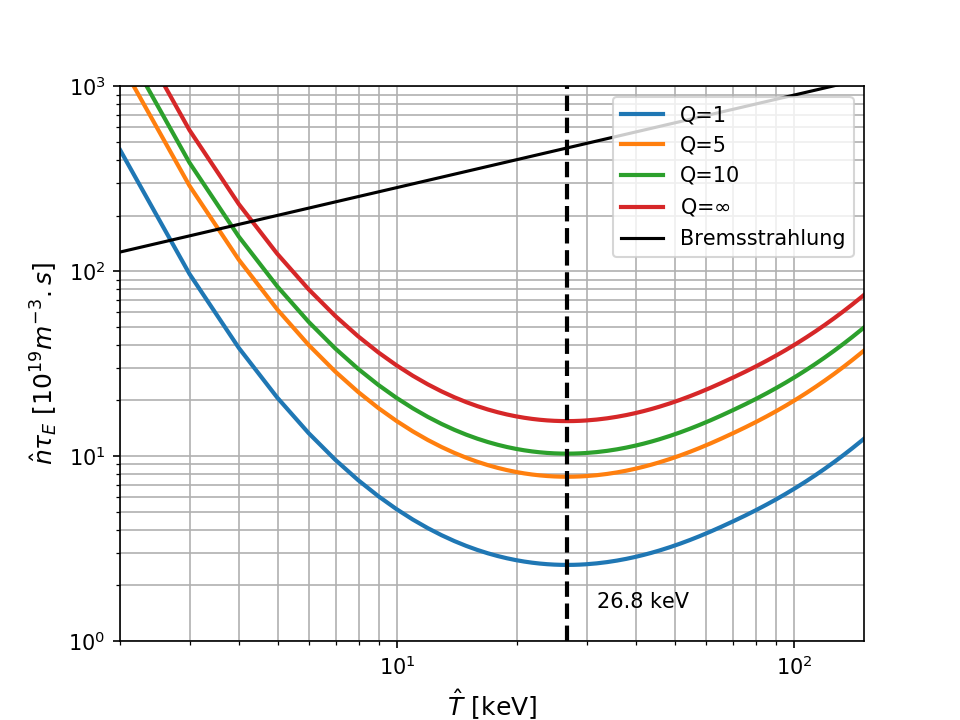
\includegraphics[width=1\textwidth]{figures/ntau_e_vs_T_loglog.png}
	\end{center}
    \caption{$\hat n \tau_E$ evaluated as a function of $\hat T$ and for different values of $Q$ ($\gamma_{rad}=1$). All curves have a minimum for $\hat T\approx 26.8$~keV. Break-even and ignition contours correspond to $Q=1$ and $Q \to\infty$ curves respectively.}
	\label{fig:ntau_E_vs_T_adv}
\end{figure}


It turns out that the product $\hat n \tau_E$ is minimum for a temperature $\hat T\approx 26.8$~keV, whatever the value of $Q$. Hence the optimal target temperature to consider for D-T reactions is around 26 keV. In particular, for ignition, one must have:
\begin{equation*}
    n \tau_E > 15 \times 10^{19} \si{\left[m^{-3} s \right]} 
\end{equation*}

In addition, another important point is the thermal stability of the regime: the total power absorbed by the system should be a decreasing function of temperature (otherwise it would lead to a temperature divergence). With this additional constraint, it appears that the minimum stable value is reached at $T\approx 15 \si{keV}$ (cf.\ref{sec:thermal_stability}).


Finally, in the temperature range $T_{\mathrm{[keV]}} \in [10.3-18.5]$ keV, it turns out that the reactivity $\left< \sigma v \right>_{DT}$ can well (with about 10$\%$ error) be approximated by \cite[(1.5.4)]{Wesson2004}: 

\begin{equation}
\left< \sigma v \right>_{DT} 
\approx 
1.18 \times 10^{-24}\; \hat T^2 \;\si{\left[m^3 s^{-1}\right]}
\end{equation}
so that the criterion for ignition becomes (assuming a flat profiles): 
\begin{equation*}
    n T \tau_E > 3 \times 10^{21} \si{\left[m^{-3} keV s \right]}
\end{equation*}


\subsubsection{Fusion Power as a function of Temperature or Beta}
All in all, one gets (in MW):
\begin{equation}
\hat P_{fus} = C_{fus} \kappa \varepsilon^2 R^3 \hat n^2 \hat T^2  
\label{eq:DT_fusion_power}
\end{equation}
with $C_{fus} \approx 17.59 \times e\times 1.18\, 10^{-24} \times 10^{2\times19}\times \pi^2/2 \approx 1.64\, 10^{-3}$. We recall here that $\hat T$ is expressed in keV, and $\hat n$ in $10^{19} \, \si{m^{-3}}$. 


The fusion power can also be expressed in terms of $\beta_N$by using eq.\ref{eqn:nT_betaN}:
\begin{equation}
\hat P_{fus} = \frac{C_{fus}C_I^2}{C_\beta^2} \frac{\kappa \varepsilon^4}{q_a^2} 
\beta_N^2 R^3 B^4 
\label{eq:DT_fusion_power_betaN}
\end{equation}



% --------------------------------------------------
% --------------------------------------------------
\subsection{Plasma Radiation}\label{sec:plasma_radiation}
In a fusion plasma, the three most important types of radiation are: 
\begin{itemize}
	\item Bremsstrahlung radiation, due to Coulomb collisions 
	\item line radiation (when the plasma contains impurity species), 
	\item cyclotron radiation, due to particle motion in a magnetic field.
\end{itemize}

Bremsstrahlung radiation is an important radiation loss in fusion plasma and usually dominates the two other radiation mechanisms for plasma temperature below then 20 keV. 



% --------------------------------------------------
% --------------------------------------------------
\subsubsection{Bremsstrahlung Radiation}
Bremsstrahlung radiation, i.e., "braking radiation" or "deceleration radiation", is the electromagnetic radiation produced by the Coulomb interactions between electrons and ions. As in fusion plasma, multiple ions species are present, the power loss density can be expressed as \cite[sec.3.3]{FusionCEA1987}, \cite[sec.4.24]{Wesson2004}, \cite[sec.3.5.4]{Freidberg2007}

\begin{equation}
S_B
=
C_B Z_{eff} n_e^2 \hat T^{1/2}
\end{equation}
with $\hat T$ in keV and where 
\begin{equation*}
C_B 
\approx
5.355 \times 10^{-37} \left[ \frac{W m^3}{ \sqrt{keV}} \right]
\end{equation*}
with $Z_{eff}$ the effective charge, representing the average
charge state of species $s$\footnote{Species do not need to be fully ionized}, defined by:
\begin{equation}
Z_{eff}
=
\frac{1}{n_e}
\sum_s
n_s Z_s^2
\label{eq:effective_charge_adv}
\end{equation}
Assuming constant density and temperature profile, one would gets:
\begin{equation}
	P_B
	=
	C_B 10^{19\times 2} 
	C_B Z_{eff} \hat n^2 \hat T^{1/2}
	V
\label{eq:Bremsstrahlung_Power_Loss}
\end{equation}

In any case, this radiation loss $P_B$ will be always lower than all the losses $P_{loss}$, ie.:
\begin{equation*}
	P_{loss} > P_B
\end{equation*}
which leads to the inequality illustrated in figure \ref{fig:ntau_E_vs_T_adv}:
\begin{equation}
	\hat n \tau_E < \frac{3\times 10^3 10^{-19} e }{C_B} \hat T^{1/2}
\end{equation}

% ---------------------------------------------------------------------------
\subsubsection{Line Radiation}
line-radiation would better account for the effects of heavy impurities that are emitted from the divertor plate and first wall.

TODO

% ---------------------------------------------------------------------------
\subsubsection{Synchrotron Radiation}

TODO


% --------------------------------------------------
% --------------------------------------------------
\subsection{MHD Instabilities}
The plasma beta $\beta$ is defined as the ratio of the plasma pressure $p=2nk_BT$ (the factor 2 comes from the fact that the total temperature is considered, $i.e.$ $n(T_e+T_i)$, with the assumption of equal ion and electron temperatures) to the magnetic pressure $B^2/2\mu_0$:
\begin{equation}
	\beta
	\doteq 
	\frac{p}{B^2/2\mu_0}
	=
	\frac{2 n k_B T}{B^2/2\mu_0}
\end{equation}
or, in terms of normalized parameters:
\begin{equation}
	\beta
	=
	C_\beta \frac{\hat n \hat T}{B^2}
\label{eqn:beta_adv}
\end{equation}
where $C_\beta = 4\mu_0\times 10^{19}\times 10^3 e \approx 0.00805$. Pay attention that we often define $\beta_\%$ as $\beta_\% \doteq 10^2\, \beta$,  expressed in $\%$.


Several modes (such as e.g. kink, tearing or ballooning modes) become MHD unstable above certain thresholds of pressure gradient and plasma current, so that one can expect that $\beta$ will be subject to a stability limitation which will likely depend on the plasma current. \emph{``However, the concept of $\beta$ limit is not precise. Stability depends on profiles, and any optimisation introduces the questions of which modes of instability to include and what mode numbers to allow. Furthermore, there is uncertainty as to the severity of the nonlinear consequences of the various modes. Nevertheless the intrinsic usefulness of a concise analytic $\beta$ limit in assessing possible tokamak performance has prompted a number of investigations''} \sidecite{Wesson2004}.

It turns out that the $\beta$ limit, i.e. the maximum stable $\beta$, scales approximately like $\varepsilon/q_a$, which can be recast as $(\mu_0/2\pi)\; I_p/aB$ from the above relations. We shall define $\beta_m$ as follows:
\begin{equation*}
\beta \leqslant \beta_m \doteq g\; \frac{\hat I_p}{a B}
\end{equation*}
The coefficient of proportionality $g$ depends on the considered instabilities. The so-called "Troyon limit" \sidecite{Troyon1984} puts this coefficient to $2.8\, 10^{-2}$ (or 2.8 if $\beta$ is expressed in $\%$).
It is usual to introduce the normalised $\beta$, called $\beta_N$, defined by Eq.(13.146) from \sidecite{Freidberg2007}:
\begin{equation}
\beta \doteq \beta_N \frac{\hat I_p}{a B}
\end{equation}
Then, the stability limit simply reads $\beta_N <g$.

% --------------------------------------------------
% --------------------------------------------------
\subsection{Density Limit - plasma pressure}
The expression of $\beta$ ()\ref{eqn:beta_adv}) can also be used to set a maximum boundary of the plasma density. Indeed, in order to get a magnetically confined plasma, one must insure that $\beta < 1$. This leads to the inequality:
\begin{equation}
    \hat n < \frac{B^2}{C_\beta \hat T}
\end{equation}

For $T=15 \si{keV}$, this leads to the following  

% --------------------------------------------------
% --------------------------------------------------
\subsection{Density Limit - Greenwald density}

As stated in a recent topical review on the subject \sidecite{Greenwald2002}, \emph{``in addition to the operational limits imposed by MHD stability on plasma current and pressure, an independent limit on plasma density is observed in confined toroidal plasmas. [...] In tokamaks, [...] there is strong evidence linking the limit to physics near the plasma boundary [...]''}. As a matter of fact, the so-called Greenwald density $n_G$ is not a sharp density limit, since discharges with peaked density profiles can well operate above this value. So far, there is no widely accepted, first principles model for the density limit. Yet, the focus is currently either on mechanisms which lead to strong edge cooling, or on collisionality enhanced turbulent transport.

From \cite[eq.(14.146)]{Freidberg2007}, the most common empirical scaling for (line-averaged) density limit is the following:
\begin{equation}
\hat n_G \doteq C_n \frac{\hat I_p}{\varepsilon^2 R^2}
\label{eqn:greenwald_density_adv}
\end{equation}
with $C_n = 10/\pi \approx 3.18$.
Using the expression of the plasma current given above, and replacing $\mu_0$ by its value, $\hat n_G$ can be recast as follows:
\begin{equation*}
\hat n_G = C_nC_I \frac{B}{q_aR}
\end{equation*}
Finally, one introduces the normalised density $n_N\doteq n/ n_G$, so that:
\begin{equation}
\hat n = C_nC_I\; n_N\; \frac{B}{q_aR}
\label{eq:n_nN_adv}
\end{equation}


% --------------------------------------------------
% --------------------------------------------------
\subsection{Scaling law exponents}
It is important to realize that the exponents of the power law are actually bound by critical relations, which derive from the invariance properties of the underlying governing equations, namely Vlasov and Maxwell's equations. These relations are sometimes called the "Kadomtsev constraints", acknowledging his decisive contribution \sidecite{Kadomtsev1975} to import in the field of fusion science the pioneering works of Buckingham on scale invariance \sidecite{Buckingham1914}\footnote{On the question of dimensional analysis applied to physics in general, see also reference \cite{Misic2010}, and references \cite{Connor1977, Luce2008} for the specific case of fusion plasmas.}. For instance, as recalled in \cite{ITERphysics_chap2} (p.2204), a standard constraint imposes the relation 
$4\alpha_R - 8\alpha_n - \alpha_I - 3\alpha_P - 5\alpha_B = 5$, with $\alpha_X$ the exponent of variable $X$ in the scaling law. The rationale is briefly recalled in Appendix~\ref{appendix:scaling_law_dimensionless}.

% --------------------------------------------------
% --------------------------------------------------
% --------------------------------------------------
\section{Expression Reformulations}\margintoc
% ------------------------------------------------------
\subsection{Plasma Pressure}
Using the expression Eq.(\ref{eq:}) and that of the plasma current Eq.(\ref{eq:plasma_current_adv}), the plasma pressure can be expressed as a function of $\beta_N$ and $B$ from Eq.(\ref{eqn:beta_adv}):
\begin{eqnarray}
\hat n\hat T &=& C_\beta^{-1} \beta_N \frac{\hat I_p B}{\varepsilon R} \nonumber \\
&=& \frac{C_I}{C_\beta}\; \frac{\varepsilon}{q_a} \;  \beta_N B^2
\label{eqn:nT_betaN_adv}
\end{eqnarray}

% ------------------------------------------------------
\subsection{Plasma Energy}
The plasma energy (\ref{eq:total_energy_natural_units}) is re-expressed in terms of normalized units: (in [MW.s]):

\begin{equation}
\hat W = 2\pi^2 C_{loss}  \varepsilon^2  \hat n \hat T R^3
\label{eq:total_energy}
\end{equation}
where $C_{loss} = 3 \times 10^{19} \times 10^{-3} e$.



% ---------------------------------------------------
\subsection{Fusion Power}
Using the expression of the reactivity for the considered range of temperature, fusion power (\ref{eq:FusionPower1}) gets (in MW):
\begin{equation}
\hat P_{fus} 
=
\frac{2\pi^2}{4}
\varepsilon^2 R^3
n^2 E_{DT}
\times
1.18\, 10^{-24-6}\; \hat T^2 
\end{equation}
or, in terms of normalized parameters:
\begin{equation}
\boxed{
	\hat P_{fus} 
	=
	C_{fus} \kappa \varepsilon^2 R^3 \hat n^2 \hat T^2
}
\label{eq:DT_fusion_power_adv}
\end{equation}
with $C_{fus} \approx 17.59 \times e\times 1.18\, 10^{-24} \times 10^{2\times19}\times \pi^2/2 \approx 1.64\, 10^{-3}$. We recall here that $\hat T$ is expressed in keV, and $\hat n$ in $10^{19} \, \si{m^{-3}}$. 



Moreover, the fusion power (\ref{eq:DT_fusion_power_adv}) can be expressed in terms of $\beta_N$by using eq.\ref{eqn:nT_betaN_adv}:
\begin{equation}
\boxed{
		\hat P_{fus} 
	= 
	\frac{C_{fus}C_I^2}{C_\beta^2} \frac{\kappa \varepsilon^4}{q_a^2} 
	\beta_N^2 R^3 B^4
}
\label{eq:DT_fusion_power_betaN_adv}
\end{equation}

\subsection{Loss Power}
The power loss can be written in terms of normalized parameters as:
\begin{equation}
	\hat P_{loss} \doteq \frac{\hat W}{\tau_E} 
	= C_{loss} \kappa \varepsilon^2  \frac{\hat n \hat T R^3}{\tau_E}
\label{eq:Ploss_adv}
\end{equation}

Similarly to what we did for the D-T fusion power, $P_{loss}$ can also be expressed as a function of $\beta_N$ (using eq.\ref{eqn:nT_betaN_adv}):
\begin{equation}
	\hat P_{loss} 
	= 
	\frac{C_{loss}C_I}{C_\beta}  \frac{\kappa \varepsilon^3}{q_a}
	\frac{\beta_N R^3 B^2}{\tau_E}
\label{eq:Ploss_betaN_adv}
\end{equation}

%------------------------------------------------------
\subsection{Triple Product}
At equilibrium, using both expressions of the powers, more precisely eq.(\ref{eq:Pnet_as_Pfus_Q}), (\ref{eq:DT_fusion_power_adv}) and eq.(\ref{eq:Ploss_adv}), one then obtains an expression for the so-called triple product $nT\tau_E$:
\begin{equation}
	\hat n \hat T \tau_E = \frac{C_{loss}}{\gamma_{rad} C_{fus}} \frac{Q}{1+Q/\lambda}
\label{eq:nTtau_Q_adv}
\end{equation}


% -----------------------------------------------------
\subsection{Confinement Time}
Introducing the normalised density $n_N = \hat n/\hat n_G$ (eq.\ref{eq:n_nN_adv}) and replacing the current by its expression eq.\ref{eq:plasma_current_adv}, the scaling law can be recast as follows:
\begin{equation*}
\tau_E = C_{SL} C_n^{0.41} C_I^{1.34} \hat M^{0.19} \kappa^{0.78} \varepsilon^{2.44} q_a^{-1.34}
n_N^{0.41} R^{2.49} B^{1.49} \hat P_{net}^{-0.69}
\end{equation*}

One last step is to replace $\hat P_{net}$ by $\hat P_{loss}$ (eq.\ref{eq:Ploss_betaN_adv}), which is equivalent at equilibrium, and to use the expression of the pressure in terms of $\beta_N$ (eq.\ref{eqn:nT_betaN_adv}) to obtain the following relation:
\begin{equation}
\boxed{
	(\hat n\hat T\tau_E)^{0.31} 
	= 
	C_{SL} C_n^{0.41} C_I^{0.96} C_\beta^{0.38} 
	C_{loss}^{-0.69}
	\hat M^{0.19} \kappa^{0.09} \varepsilon^{0.68} q_a^{-0.96}
	n_N^{0.41} R^{0.42} B^{0.73} \beta_N^{-0.38}
}
\label{eq:nTtau_betaN_adv}
\end{equation}
The left hand side is fully determined by the value of $Q$, cf. Eq.(\ref{eq:nTtau_Q_adv}). \\

In turn, Eq.(\ref{eq:nTtau_betaN_adv}) provides an expression of $\beta_N$ as a function of $R$, $B$ and $Q$ at prescribed values of the average ion mass $\hat M$, of geometrical variables ($\kappa$ and $\varepsilon$), of the edge safety factor $q_a$ and of the normalised density $n_N$.
Equation (\ref{eq:DT_fusion_power_betaN_adv}) is the other independent relation for $\beta_N$, expressed as a function of $R$, $B$ and $P_{fus}$ (again at prescribed $\kappa$, $\varepsilon$ and $q_a$).




% --------------------------------------------------
% --------------------------------------------------
% --------------------------------------------------
\section{Searching for a solution}
The equation (\ref{eq:DT_fusion_power_betaN_adv}) can be restated as:

\begin{equation}
	R^3 B^4 
	=
	\frac{
		\hat P_{fus}
	}{
		\frac{C_{fus}C_I^2}{C_\beta^2} \frac{\kappa \varepsilon^4}{q_a^2} 
		\beta_N^2 
	}
\end{equation}
and the equation (\ref{eq:nTtau_betaN_adv}), in association with equation (\ref{eq:nTtau_Q_adv}), can also be recasted as:
\begin{equation}
R^{0.42} B^{0.73}
=
\frac{
	\left( 
		\frac{C_{loss}}{\gamma_{rad} C_{fus}} \frac{Q}{1+Q/\lambda} 
	\right)^{0.31} 
}{
	C_{SL} C_n^{0.41} C_I^{0.96} C_\beta^{0.38} 
C_{loss}^{-0.69}
\hat M^{0.19} \kappa^{0.09} \varepsilon^{0.68} q_a^{-0.96}
n_N^{0.41}  \beta_N^{-0.38}
}
\end{equation}

These two solutions should be solved together for a prescribed value of $\beta_N$. An other possibility is to deduce the $(R,B)$ map of $\beta_N$ using these two expressions, and to seek for common solutions of $\beta_N$ to deduce a couple $(R,B)$.

 

% --------------------------------------------------
% --------------------------------------------------
% --------------------------------------------------
\section{Additional discussions}\margintoc
The model which has been derived can be made more realistic, taking into account the following additional parameters, described in the next subsections.


% -------------------------------------------------------
\subsection{Peaking factors}
In reality, density and temperature are not constant but are function of the radial position in the plasma. During spatial integrations in the later derivations, a more realistic profile could have been used. Realistic profiles can be described as parabolic profiles, which can be defined for density and temperature as:

\begin{align}
	n(\rho)
	=&
	\left< n \right>
	\left(1 + \nu_n \right)
	\left(1 + \rho^2 \right)^{\nu_n}
	\\
	T(\rho)
	=&
	\left< T \right>
	\left(1 + \nu_T \right)
	\left(1 + \rho^2 \right)^{\nu_T}
\end{align}
where $\nu_n$ and $\nu_T$ are peaking factors and $\left< n \right>$ and $\left< T \right>$ the volume averaged density\sidenote{\begin{equation*}
	\left< n \right> =
	\frac{1}{V}
	\int n(r) dr
	\end{equation*} } 
and temperature respectively. The profiles are prescribed in terms of $\rho$, a normalized radial-like flux coordinate, with $\rho=0$  at the magnetic axis and $\rho=1$ at the outer plasma surface.

Let's define a peaking factor of the temperature profile
\begin{equation}
	f_{pT}
	\doteq
	\frac{\left< T^2 \right>}{\left< T \right>^2}
\end{equation}


% -------------------------------------------------------
\subsection{Fraction of $\alpha$ particles}
Assuming that the plasma contains only deuterium, tritium and $\alpha$ (He) particles, 
Let's define the ratio of $\alpha$ particles as:
\begin{equation}
f_\alpha
\doteq
\frac{n_{He}}{n_e}
\end{equation}

dilution factor $f_D$ $n_D = n_T = f_D \left( \frac{n}{2} \right)$. 


% -------------------------------------------------------
\subsection{Ratio of ion to electron temperature}


% -------------------------------------------------------
\subsection{Other points}
\begin{itemize}
	\item pulsed or steady-state device ? This needs discussion on bootstrap current, current density profile
	\item Radiation losses
\end{itemize} 




%==============================================
\section{Dimensioning a Tokamak}
%==============================================
From the previous equations mostly derived from a 0-dimensional approach (shaped profiles have not been considered so far), a suitable couple $(R, B)$ may be found for a given reactor project of prescribed $(P_{fus}, Q)$. By proceeding this way, some other characteristics of the plasma (namely the shape of the plasma, including elongation and aspect ratio, the average ion mass $\hat M$, the edge safety factor $q_a$ and the density $n_N$ normalised to the Greenwald density) are assumed to be prescribed by other considerations. Notice however that these other variables actually offer additional degrees of freedom to the exercise. The method is applied to the ITER case in section \ref{sec:ITER_spec}.

Should such a $(R, B)$ couple be found, additional important questions then arise before deciding whether it effectively constitutes a suitable tokamak. These includes, but are not limited to, the issues of superconducting magnets with their cryostat and neutron shielding, the issue of power exhaust and of the maximum affordable heat flux per square meter, the capacity to sustain a sufficiently long a plateau of plasma current...\\

%----------------------------------------------
\subsection{Recovering ITER specifications}
\label{sec:ITER_spec}

The objective here is to find a suitable couple of major radius and magnetic field $(R,B)$ which would allow one to reach the ITER targets in terms of fusion gain $Q=10$ and fusion power $\hat P_{fus}=500$ MW.
So as to get closer to the actual specifications of ITER, one should first refine the various constants introduced in section \ref{sec:governing_eqs}. One introduces the following refinements:
\begin{enumerate}
    \item $f_\alpha \doteq n_{He}/n_e$ the fraction of $\alpha$ particles
    \item $f_p \doteq \langle T^2 \rangle / \langle T \rangle^2$ the peaking factor of the temperature profile (a flat density profile is assumed). Here and hereafter in this section, the brackets $\langle ...\rangle$ refer to volume averaged quantities.
    \item $\theta_i \doteq T_i/T_e$ the ratio of ion to electron temperatures
\end{enumerate}
Several coefficients are modified by these additional variables:
\begin{eqnarray*}
    && C_{fus} \to C_{fus} \times (1-2f_\alpha)^2\theta_i^2 \times f_p \\
    && C_{loss} \to C_{loss} \times \frac{1+\theta_i - f_\alpha\theta_i}{2}  \\
    && C_\beta \to C_\beta \times \frac{1+\theta_i - f_\alpha\theta_i}{2}
\end{eqnarray*}
The corrections regarding $C_{fus}$ result from the fact that $P_{fus}$ scales like $\langle n_Dn_TT_i^2 \rangle$, with $n_D = n_T = 0.5\; (1-2f_\alpha)n_e$ so as to fulfill electro-neutrality ($n_D+n_T+2n_{He}=n_e$), and $\langle T_i^2 \rangle = f_p\; \langle T_i \rangle^2$ by definition. As expected, $\alpha$ particles are responsible for a dilution effect. The correction regarding $C_{loss}$ and $C_\beta$ is due to the fact that both the power loss and $\beta$ scale like the total pressure which reads: $\sum_s n_sT_s = n_eT_e (1+\theta_i- f_\alpha \theta_i)$ with the assumption that $T_\alpha=T_i$.
In addition, the effective mass $\hat M$ simply derives from $f_\alpha$\footnote{Indeed, one has: $(n_D+n_T+n_{He})\; \hat M \doteq n_D\hat M_D + n_T\hat M_T + n_{He}\hat M_{He} =
n_e\left\{ (\hat M_D + \hat M_T)(1-2f_\alpha)/2 + f_\alpha \hat M_\alpha \right\}$, with $\hat M_D=2$, $\hat M_T=3$ and $\hat M_\alpha=4$.}:
\begin{equation*}
    \hat M = \frac{5  - 2f_\alpha}{2(1-f_\alpha)}
\end{equation*}
Finally, geometrical effects modify the $C_I$ coefficient. When including the effect of triangularity $\delta$, the revised expression reads as follows (cf. eq.(17) in \cite{Johner2011}):
\begin{equation*}
    C_I \to C_I \times 
    \frac{(1.17-0.65\, \varepsilon)\; \left[ 1+\kappa^2(1+2\delta^2-1.2\delta^3) \right]} {2\;(1-\varepsilon^2)^2}
\end{equation*}

\begin{figure} 
	\begin{center}
		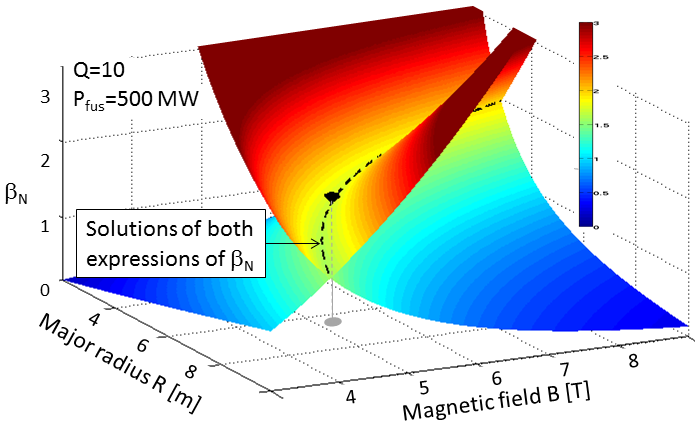
\includegraphics[width=0.8\textwidth]{figures/Fig_3D_betaN_R_B_ITER_v3.png}
		\caption{Surfaces governed by eq.\ref{eq:DT_fusion_power_betaN} and eq.\ref{eq:nTtau_betaN} in the 
			3-dimensional $(\beta_N,R,B)$ space. Black dashed line: intersection of these 2 surfaces.}
		\label{fig:R_B_betaN_3D}
	\end{center}
\end{figure}

\begin{figure} 
	\begin{center}
		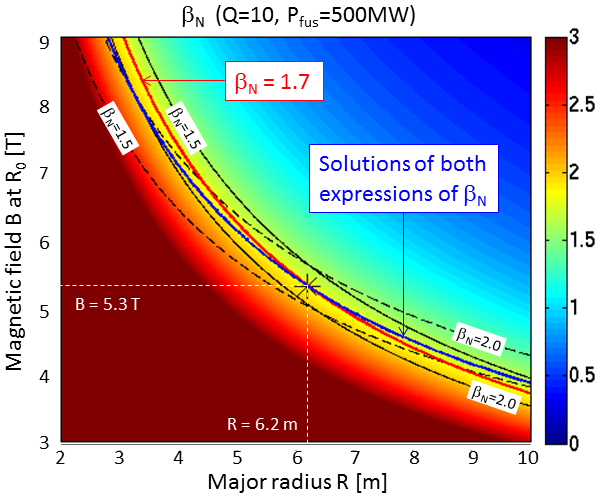
\includegraphics[width=0.7\textwidth]{figures/Fig_2D_betaN_R_B_ITER_v3.png}%\hfill
		%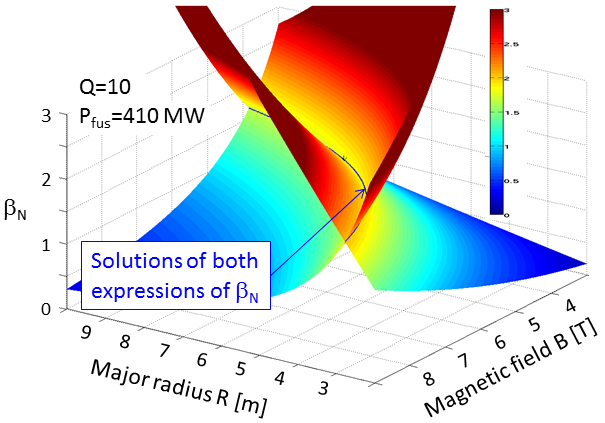
\includegraphics[width=0.5\textwidth]{figures/Fig_3D_betaN_R_B_ITER.png}
		\caption{Map of $\beta_N=f(R,B)$ given by eq.\ref{eq:DT_fusion_power_betaN} (color-scale and plain contour lines) and eq.\ref{eq:nTtau_betaN} (dashed contour lines). Blue line: intersection of these 2 surfaces. Red line: $\beta_N = 1.7$.}
		\label{fig:R_B_betaN_2D}
	\end{center}
\end{figure}

Hereafter, the following set of parameters has been considered, mostly taken from ref.\cite{Johner2011}\footnote{The chosen peaking factor would correspond, for instance, to the following temperature profile: $T = (T_0-T_a)*(1-\rho^2)^{1.18} + T_a$, with $\rho=r/a$, and $\hat T_a=0.1$ keV and  $\hat T_0=15$ keV the temperatures at the separatrix and on the magnetic axis, respectively.}:
\begin{center}
	\begin{tabular}{c|c|c|c|c|c|c|c|c}
		\hline
		$q_a$ & $\varepsilon^{-1}$ & $\kappa$ & $\delta$ & $n_N$ & $f_\alpha$ & $f_p$ & $\theta_i$ & $\gamma_{rad}$ \\
		\hline
		$3$   & $3.1$ & $1.7$ & $0.33$ & $0.85$ & $0.035$ & $1.4$ & $1/1.2$ & $0.7$ \\
		\hline	
	\end{tabular}
\end{center}
The approximate values of the various coefficients are then the following:
\begin{center}
	\begin{tabular}{c|c|c|c|c|c|c}
		\hline
		$C_{SL}$ & $C_n$ & $C_I$ & $C_\beta$ & $C_{loss}$ & $C_{fus}$ & $\hat M$ \\
		\hline
		$0.0562$ & $3.183$ & $13.144$ & $0.726$ & $0.086$ & $1.38\,10^{-3}$ & $2.55$ \\
		\hline	
	\end{tabular}
\end{center}
\bigskip

\begin{figure} 
	\begin{center}
		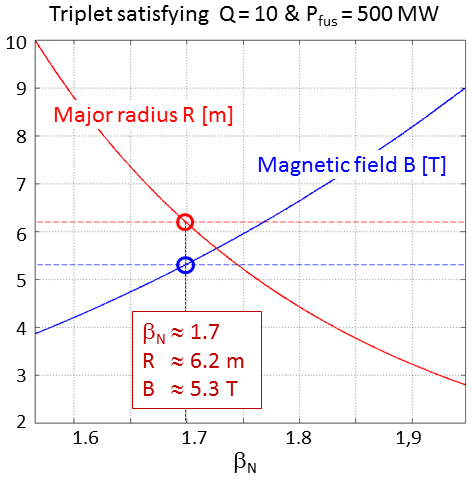
\includegraphics[width=0.5\textwidth]{figures/Fig_R_B_betaN_solutions_v3.png}
		\caption{Values of $R$ and $B$ as a function of $\beta_N$ which fulfill both equations eq.\ref{eq:DT_fusion_power_betaN} and eq.\ref{eq:nTtau_betaN} (taken along the blue line of fig.\ref{fig:R_B_betaN_2D}). The solution at $\beta_N \approx 1.7$ is close to the ITER specifications $R_{ITER}=6.2$m, $B_{ITER}=5.3$T.}
		\label{fig:solutions_betaN}
	\end{center}
\end{figure}

Two independent expressions of $\beta_N$ with respect to $R$ and $B$ are provided by equations eq.\ref{eq:DT_fusion_power_betaN} and eq.\ref{eq:nTtau_betaN}. The intersection of these 2 surfaces draws a line in the $(R,B,\beta_N)$ plane, as evident on Fig.\ref{fig:R_B_betaN_3D}. This line is plotted in blue on figures \ref{fig:R_B_betaN_3D} and \ref{fig:R_B_betaN_2D} (the latter figure being a projection of the former one). As expected, it does not follow an iso-$\beta_N$ contour (should it be the case, this would actually mean that the 2 equations are degenerate). Figure \ref{fig:R_B_betaN_2D} also shows the iso-contour lines $\beta_N \in \{1.5, 2\}$, which allow one to locate the ITER relevant region in the $(R,B)$ plane, i.e. those solutions exhibiting an acceptable $\beta_N$ value for ITER performing discharges. 
It readily appears from Fig.\ref{fig:R_B_betaN_3D} that $\beta_N$ given by eq.\ref{eq:DT_fusion_power_betaN} decreases with $(R,B)$, while eq.\ref{eq:nTtau_betaN} leads to the increase of $\beta_N$ with $(R,B)$, all other parameters being kept constant.
Noticeably, plain and dashed iso-contours look almost tangent to each other. This property implies that the set of couples $(R,B)$ which are solutions of the problem does not cover a broad range of $\beta_N$ values. This point is evident on fig.\ref{fig:solutions_betaN}, which displays the $(R,B)$ solutions as a function of $\beta_N$: for $\beta_N$ in the range $1.57 \leq \beta_N \leq 1.94$, the acceptable couples $(R,B)$ are in the range $2.85 \leq R_{[m]} \leq 9.82$ and $3.90 \leq B_{[T]} \leq 8.88$.

Interestingly, it turns out that the triplet $(R_{[m]},B_{[T]},\beta_N) = (6.2, 5.3, 1.7)$ is a possible solution of the problem\footnote{More precisely, the couple $(R_{[m]},B_{[T]}) \approx (6.200, 5.298)$ is solution at $\beta_N \approx 1.698$.}. This set of parameters is consistent with ITER specifications. \\

As evident on fig.\ref{fig:solutions_betaN}, there is \emph{a priori} an infinity of possible triplet solutions $(R,B,\beta_N)$. It appears that $B$ increases with $\beta_N$, while $R$ decreases. Basically, as will become clear in the following, large values of  $\beta_N$ are constrained by the so-called ``radial built'' -- i.e. the necessity to have sufficient space to put the central solenoid, the superconducting coils, the vacuum vessel and the necessary neutron shields -- while small values reveal too costly -- the price scales typically like $R^3$.

These additional constraints have led to the specific choice made for ITER, as a compromise. They are detailed in the next sections.


%----------------------------------------------
\subsection{Power exhaust capabilities}
\label{sec:power_exhaust}

\subsubsection*{The case without radiation}

Heat is basically transported via convection, conduction (understood here as any mechanism leading to heat transport in the absence of particle transport, except radiation) or radiation. 
Assuming no radiation at all, the plasma power loss is equal to the heating power at equilibrium. In the case of ITER, taking $P_{fus}=500\,$MW and $Q=10$, and assuming that the radiated power in the core corresponds to about $30\%$ of the total heating power ($\gamma_{rad}=0.7$), one gets $P_{loss} = \gamma_{rad} P_{fus}(1/\lambda + 1/Q) \approx 106\,$MW. \\

Assuming homogeneous power deposition in the toroidal direction, and accounting for the 2 legs of the diverted field lines, a rough estimate of the average power flux $Q_{loss}$ on the divertor target plates is given by the ratio of the loss power over the wetted area:
\begin{equation}
  \hat Q_{loss} \approx \frac{\hat P_{loss}}{4\pi R \lambda_q} \;\sin\alpha \;\;\;\; [\textrm{MW.m}^{-2}]
\end{equation}
where $\lambda_q$ stands for the radial e-folding length of the heat flux in the scrape-off layer (SOL) and $\alpha$ is the tilt angle of the plates with respect to the magnetic field lines.
Eich and co-authors have obtained an empirical scaling law for $\lambda_q$ \cite{Eich2011,Eich2013}:
\begin{equation}
  \lambda_q = 7.3\,10^{-4}\; B^{-0.78} \, q_{a}^{1.2} \, \hat P_{SOL}^{0.1}\;\;\;\; [\textrm{m}]
\end{equation}
with $\hat P_{SOL}$ the heat power crossing the separatrix.\\

Taking $\hat P_{SOL} = \hat P_{loss}$, one then gets $\lambda_q \approx 1.2\,$mm and:
\begin{equation*}
  \hat Q_{loss} \approx \frac{10^4}{29.2\, \pi} 
    \frac{\hat P_{loss}^{0.9} \, B^{0.78}}{q_a^{1.2} \, R} \;\sin\alpha
\end{equation*}
With the parameters of ITER, and taking $\alpha = 2\, \pi/180$ as a commonly retained value, this yields $\hat Q_{loss} \approx 40\,$MW.m$^{-2}$. This value exceeds the technological limit of present actively cooled materials, which is about $10\,$MW.m$^{-2}$ in steady state conditions. One of the solutions consists in injecting light impurities so as to radiate a large amount of the power in the SOL.


\subsubsection*{Injecting impurities to radiate}

%----------------------------------------------
\subsection{Radial built for superconducting magnets}
\label{sec:radial_built}


%----------------------------------------------
\subsection{Considerations regarding the cost}
\label{sec:cost}



\printbibliography[title=Bibliography]% , prenote=bibnote]

%==============================================
\section*{Acknowledgements}
%==============================================
The authors acknowledge the pioneering works of Jean Johner in this field and the helpful expertise of Jean-Luc Duchateau. The present lecture is much inspired from their early contributions to this topic.
We also wish to acknowledge the active and insightful contribution of JL Duchateau to the scientific discussions in the preparation of this document.


\newpage

%==============================================
\appendix
%==============================================
\section{Fusion power and momentum conservation}
\label{appendix:fusion_power}

Deuterium-tritium fusion reactions result from inelastic collisions, for which momentum is conserved, not energy. The total kinetic energy release for a single reaction amounts to $\hat E_0 = 17.59$MeV. So as to evaluate the fraction of energy carried out by the neutron, relativistic corrections have to be taken into account. The method is detailed below. \\

Let's admit that it is sufficient to account for relativistic corrections for neutrons only\footnote{Within the classical framework, one would predict that the neutron carries 4 fifth of the total energy, i.e. about $\hat E_n \approx 14.07$MeV. At this energy, it turns out that the velocity of neutrons reaches approximately 17\% of the speed of light ($v_n/c = (2.10^6e\hat E_n/m_n)^{1/2}/c \approx 0.17$). Relativistic corrections cannot be ignored in this case. Conversely, heavier $\alpha$ particles move at about 4\% the speed of light. Relativistic corrections can be neglected for them.}. $\alpha$ particles will be treated within the classical framework.
Momentum conservation then reads:
\begin{equation}
    m_n \gamma_n v_n = m_\alpha v_\alpha
    \label{eq:conserv_momentum}
\end{equation}
with $\gamma_n = (1-v_n^2/c^2)^{-1/2}$ the Lorentz factor for the neutrons. In the limit $v_n/c \ll1$,  $\gamma_n$ can be Taylor expanded, so that eq.\ref{eq:conserv_momentum} can be recast as follows:
\begin{equation}
    u \left( 1+\frac{\epsilon}{2}\; u^2 \right) 
    = 1
    \label{eq:conserv_momentum2}
\end{equation}
with $u \doteq v_n/(\mu v_\alpha)$, $\mu \doteq m_\alpha/m_n$ and $\epsilon \doteq \mu (v_\alpha/c)\ll1$. It is sufficient to look for perturbative solutions of the form: 
$$ u = u_0 + u_1 \;\;\; \textrm{with} \;\; u_1\ll u_0 $$
The leading order yields $u_0=1$. At next order, one readily finds:
$$ u_1 = -\frac{\epsilon^2}{2} \; u_0^3 $$
So that, in the end:
\begin{equation*}
    v_n \simeq \mu v_\alpha \left( 1-\frac{\epsilon^2}{2}\right)
\end{equation*}
where we recall that $\mu=m_\alpha/m_n$.
The kinetic energy of the neutron can then be expressed as a function of the one of the $\alpha$ particle:
\begin{eqnarray*}
    E_n &=& m_nc^2(\gamma_n-1) \approx 
    \frac{1}{2} m_nv_n^2\left[ 1+ \frac{3}{4}\frac{v_n^2}{c^2}\right] \nonumber \\
    &\approx& \mu\; E_\alpha \left( 1-\frac{\epsilon^2}{4}\right)
\end{eqnarray*}

The kinetic energy of the $\alpha$ particle $E_\alpha$ can then be expressed as a function of the total energy $E_0$ ($E_0 =E_\alpha + E_n$). Elementary algebra leads to the following relation:
\begin{equation}
    E_\alpha^2 - \frac{2(1+\mu)}{\mu^2}E_{n0}\, E_\alpha + \frac{2}{\mu^2}\; E_{n0}E_0 = 0
\end{equation}
where $E_{n0} = m_nc^2$ stands for the mass energy of the neutron. We have used the relation $\epsilon^2 = 2\mu\; E_\alpha/E_{n0}$. The only acceptable solution is\footnote{Notice that, at leading order in $E_0/E_{n0}\ll1$, this solution simply reduces to $E_\alpha \approx E_0/(1+\mu)$.}:
\begin{equation}
    E_\alpha = \frac{1+\mu}{\mu^2}
    \left( 1 - \sqrt{1-\frac{2\mu^2}{(1+\mu)^2}\frac{E_0}{E_{n0}}}\right)\; E_{n0}
\end{equation}
When performing the numerical calculation, it should be warned that $\mu\neq 4$. 
Indeed, the mass of the $\alpha$ particle is slightly less than the sum of its components (actually, this mass difference $\Delta m \approx 0.0187\; m_p$ is the one which leads to the energy release of the D-T fusion reaction $E_0 = \Delta m\;c^2$). The masses can be found in reference \cite{Wesson2004}. In particular, $m_n \approx (1+0.001378)\, m_p$ and:
%$$
%    m_n \approx (1+0.001378)m_p \;\;\; ; \;\;\; 
%    m_\alpha = 2(m_n+m_p) \approx (1-0.027404)m_p \approx 3.967\; m_n
%$$
$$
    \mu \doteq \frac{m_\alpha}{m_n} \approx (1-0.027404)\; \frac{m_p}{m_n} \approx 3.967
$$
With these data, one finally obtains $E_0/E_\alpha \approx 4.94$ and $\hat E_\alpha \approx 3.56\,$MeV, which corresponds to the published value.  

%==============================================
\section{Constraint on the scaling laws}
\label{appendix:scaling_law_dimensionless}

When expressed in engineering variables, the scaling laws for the energy confinement time usually take the following generic form (cf. eq.~\eqref{eq:scaling_law_IPB98(y,2)}):
\begin{equation}
  \label{eq:tauE_SL_generic_a}
  \tau_E \propto \hat M^{\alpha_M} \kappa^{\alpha_\kappa} \varepsilon^{\alpha_\epsilon} \hat n^{\alpha_n} \hat I_p^{\alpha_I} R^{\alpha_R} B^{\alpha_B} \hat P_{net}^{\alpha_P}
\end{equation}
First replacing $\hat I_p$ and $\hat P_{net} = \hat P_{loss}$ by their expressions eqs.~\eqref{eqn:plasma_current} and \eqref{eq:Ploss}, and considering the energy confinement time normalized to the cyclotron frequency $\omega_c = (e/m_p)\, B/\hat M$, eq.~\eqref{eq:tauE_SL_generic_a} yields:
\begin{equation}
\label{eq:tauE_SL_generic_b}
  \omega_c \tau_E \propto 
  \hat M^{\gamma\alpha_M - 1} 
  \kappa^{\gamma(\alpha_\kappa+\alpha_P)} 
  \varepsilon^{\gamma(\alpha_\epsilon+2\alpha_I+2\alpha_P} 
  \hat q^{-\gamma\alpha_I} 
  R^{\gamma(\alpha_R+\alpha_I+3\alpha_P)} 
  B^{1 + \gamma(\alpha_B+\alpha_I)} 
  \hat T^{\gamma\alpha_P}
  \hat n^{\gamma(\alpha_n+\alpha_P)} 
\end{equation}
where the following definition has been introduced:
$$ 
  \gamma \doteq \frac{1}{1+\alpha_P}
$$

Scale invariance properties play a major role in physics: by determining which transforms leave invariant the underlying equations, one can constrain the structure of some key quantities. Especially, as stated in \cite{Connor1977}: ``if the basic equations of plasma behavior [...] are invariant under a certain group of transformations, then any scaling law derived from these equations must be invariant under the same groups of transformations. It turns out that for all the conventional plasma models, this invariance property greatly circumscribes the permissible scaling laws. In other words, even though the necessary non-linear theory may be quite intractable, the mere fact that a scaling law is, in principle, derivable \emph{from certain basic equations} already provides information about that scaling law''.

Now, as we shall see, this property imposes some constraints on the exponents of the scaling law, when expressed in dimensional (or engineering) variables (like eq.~\ref{eq:tauE_SL_generic_a}). \\

Based on the fact that the system from which the energy confinement scaling law is derived obeys Vlasov' and Maxwell's equations, it can be shown that the associated physics can be described by a reduced set of independent dimensionless parameters, among which the normalized gyro-radius $\rho_*$, the plasma $\beta$ and the collisionality $\nu_*$ \cite{Kadomtsev1975, Connor1977}. In that spirit, all dimensional engineering variables entering the scaling of $\tau_E$ (namely $R$, $B$, $\hat n$ and $\hat T_e$) should be able to be recast as functions of $\rho_*$, $\beta$ and $\nu_*$ only when expressed in terms of the dimensionless quantity $\omega_c \tau_E$ (cf. eqs.(14-16) of ref.\cite{ITERphysics_chap2}):
\begin{eqnarray}
  \rho_*  &\doteq& \left( \frac{2.10^3 m_p}{e} \right)^{1/2}\; \frac{(\hat M \hat T_i)^{1/2}}{\varepsilon R B} \\
  \beta   &\doteq& 2.10^{22}e\mu_0\; \frac{\hat n(\hat T_e+\hat T_i)}{B^2} \\
  \nu_*   &\doteq& \nu_{ii}\; \frac{qR \varepsilon^{-3/2}}{(10^3e\, \hat T_i/\hat M m_p)^{1/2}}
   = \frac{4.10^{13}\sqrt{\pi}\,e}{3} \frac{\ln\Lambda}{(4\pi\varepsilon_0)^2}\; 
     Z^4 qR \varepsilon^{-3/2}\; \frac{\hat n}{\hat T_i^2}
\end{eqnarray}
which also reads, regarding critical dependencies:
\begin{eqnarray}
\rho_*  &\propto& \frac{(\hat M \hat T_e \theta_i)^{1/2}}{\varepsilon R B} \\
\beta   &\propto& \frac{\hat n\hat T_e(1+\theta_i)}{B^2} \\
\nu_*   &\propto& Z^4 qR \varepsilon^{-3/2}\; \frac{\hat n}{f_p \theta_i^2\hat T_e^2}
\end{eqnarray}
After some tedious yet simple calculus, one gets the following relations:
\begin{eqnarray}
\hat T_e &\propto& \left( \frac{B\beta}{\rho_*\nu_*} \right)^{2/5} \; 
 \left\{ \frac{qZ^4}{f_p(1+\theta_i)} \left(\frac{\hat M}{\varepsilon^5\theta_i^3}\right)^{1/2} \right\}^{2/5} \\
\hat n   &\propto& \left( B^8\rho_*^2\nu_*^2\beta^3 \right)^{1/5} \;
 \left\{ \frac{q^2Z^8(1+\theta_i)^3}{f_p^2} \frac{\hat M}{\varepsilon^5\theta_i^3} \right\}^{-1/5}\\
R        &\propto& \left( \frac{\beta}{\rho_*^6\nu_*B^4} \right)^{1/5}\;
\left\{ \frac{qZ^4}{f_p(1+\theta_i)} \frac{\hat M^3\theta_i}{\varepsilon^{15/2}} \right\}^{1/5}
\end{eqnarray}
from which it follows that eq.\ref{eq:tauE_SL_generic_b} also reads (here, we only retain the main dimensionless parameters discussed in the literature, namely $\rho_*$, $\beta$, $\nu*$, $\hat M$, $q$, $\varepsilon$ and $\kappa$): 
\begin{eqnarray}
\label{eq:tauE_SL_generic_dimensionless}
\omega_c \tau_E \propto &&
B^{\gamma(5+3\alpha_P+5\alpha_B+\alpha_I-4\alpha_R+8\alpha_n)/5} \nonumber\\
%Z^{4\gamma(\alpha_R+\alpha_I+3\alpha_P-2\alpha_n)/5} \;
%f_p^{\gamma(-\alpha_R-\alpha_I-3\alpha_P+2\alpha_n)/5} \;
%(1+\theta_i)^{\gamma(-\alpha_R-\alpha_I-8\alpha_P-3\alpha_n)/5} \;
%\theta_i^{\gamma(\alpha_R+\alpha_I+3\alpha_P+3\alpha_n)/5} \;
&&
\rho_*^{\gamma(-6\alpha_R-6\alpha_I-18\alpha_P+2\alpha_n)/5} \;
\nu_*^{\gamma(-\alpha_R-\alpha_I-3\alpha_P+2\alpha_n)/5} \;
\beta^{\gamma(\alpha_R+\alpha_I+8\alpha_P+3\alpha_n)/5}  \nonumber\\
&&
\hat M^{\gamma(5\alpha_M+3\alpha_R+3\alpha_I+9\alpha_P-\alpha_n)/5 - 1}  \;
\hat q^{\gamma(-4\alpha_I+\alpha_R+3\alpha_P-2\alpha_n)/5}  \nonumber\\
&&
\varepsilon^{\gamma(\alpha_\epsilon+\alpha_I/2-3\alpha_R/2-5\alpha_P/2+\alpha_n)}  \;
\kappa^{\gamma(\alpha_\kappa+\alpha_P)} 
\end{eqnarray}
Now, it becomes clear that the scaling exponent of $B$ should vanish, so as to preserve the dimensionless character of $\omega_c \tau_E$ (and the subsequent fact that it should not depend on the choice of units for $B$). This constraint, sometimes referred to as the Kadomtsev constraint, leads to the following relationship:
$$
5+3\alpha_P+5\alpha_B+\alpha_I-4\alpha_R+8\alpha_n = 0
$$
When applied to the scaling exponents of the ITER IPB98(y,2) scaling law eq.\ref{eq:scaling_law_IPB98(y,2)}, this relation yields: $5-3\times 0.69+5\times0.15+0.93-4\times1.97+8\times0.41 = 0.01 \approx 0$, as expected. Expressed in dimensionless variables, this scaling law then reads as follows:
\begin{equation}
\label{eq:scaling_law_IPB98(y,2)_dimensionless}
\left. \omega_c \tau_E \right|_{IPB98(y,2)}\propto 
\rho_*^{-2.68} \;
\nu_*^{-0.01} \;
\beta^{-0.90} 
\hat M^{0.95} \;
\hat q^{-2.99}  \;
\varepsilon^{0.73}  \;
\kappa^{0.29} \;
\end{equation}
This expression is consistent with eq.(21) of ref.\cite{ITERphysics_chap2}\footnote{Actually, eq.(21) of ref.\cite{ITERphysics_chap2} exhibits a slightly different form, since $\tau_E$ is expressed as function of the Bohm time $\tau_B \propto \varepsilon^2R^2B\hat T_i^{-1}$. Notice that $\omega_c\tau_B \propto \rho_*^{-2}$. Also, the scaling exponent of $\kappa$ is wrong (cf. $e.g.$ [D. McDonald, Nuclear Fusion 47 (2007) 147], p.167, eq.(8)): it should read $\alpha_\kappa = 3.3$. Then, replacing $C_I$ by $\kappa C_I$ in our calculations, as suggested by eq.(17) of ref.\cite{ITERphysics_chap2}, one then finds that the $\kappa$ exponent in eq.\ref{eq:tauE_SL_generic_dimensionless} should read $\gamma(\alpha_\kappa+\alpha_P+\alpha_I)$ (instead of $\gamma(\alpha_\kappa+\alpha_P)$). As expected, it is equal to 3.29 in this case.}. In particular, notice the strong dependency of the energy confinement time with respect to $\rho_*$. This power coefficient, close to 3, is reminiscent of the so-called \emph{gyro-Bohm} transport, where the effective turbulent diffusivity scales like $\chi_\perp \sim \rho_* \chi_{B}$, with $\chi_B = T/eB$ the Bohm diffusion coefficient. This unfavorable scaling explains why large performance gains can only be achieved in large machines, like ITER.

\end{document}
